\documentclass{article}
\usepackage{amsmath}
\usepackage{amsfonts}
\usepackage{amssymb}
\usepackage{hyperref}
\usepackage{graphicx}

\usepackage{xcolor}
\usepackage{enumitem}
\usepackage{geometry}
\geometry{a4paper, margin=1in}

\usepackage{theorem}

\usepackage{float}
\usepackage{booktabs}

\usepackage{algorithm,algpseudocode}
\usepackage{algorithm}

\usepackage{url}
\PassOptionsToPackage{hyphens}{url}\usepackage{hyperref}

\usepackage{caption}

\usepackage{listings}
\usepackage{color}

\definecolor{codegreen}{rgb}{0,0.6,0}
\definecolor{codegray}{rgb}{0.5,0.5,0.5}
\definecolor{codepurple}{rgb}{0.58,0,0.82}
\definecolor{backcolour}{rgb}{0.99,0.99,0.99}

\lstdefinestyle{mystyle}{
    backgroundcolor=\color{backcolour},   
    commentstyle=\color{codegreen},
    keywordstyle=\color{magenta},
    numberstyle=\tiny\color{codegray},
    stringstyle=\color{codepurple},
    basicstyle=\ttfamily\footnotesize,
    breakatwhitespace=false,         
    breaklines=true,                 
    captionpos=b,                    
    keepspaces=true,                 
    numbers=left,                    
    numbersep=5pt,                  
    showspaces=false,                
    showstringspaces=false,
    showtabs=false,                  
    tabsize=2
}

\usepackage[utf8]{inputenc}

\usepackage[backend=biber, style=authoryear, citestyle=authoryear]{biblatex}

\lstset{style=mystyle}

{
\title{
    \includegraphics[width=0.31\textwidth]{/Users/mlnick/documents/Logos_and_pics/TSUKUBA_logo.png} \\
    \vspace{3mm}
    \textbf{Evolution of SALSA-type Attacks on LWE} \\
    \vspace{3mm}    
    CryptoSemi proceeding
}

\author{Mamanchuk Mykola, SID.202420671}
\date{\today}

\begin{document}
\maketitle

\section{Introduction to SALSA-type Attack Improvements}

\textbf{Objective}: This section presents the progression and key improvements of SALSA-type attacks on the Learning With Errors (LWE) problem, focusing on the advancements made from the original SALSA (Secret-recovery Attacks on LWE via Sequence to sequence models with Attention) to SALSA PICANTE and SALSA VERDE. These attacks leverage machine learning techniques, particularly transformer models, to recover secrets in LWE instances, demonstrating significant advancements in cryptanalysis of LWE-based cryptosystems.

\subsection{Key Improvements in SALSA Concepts}

The SALSA family of attacks represents a significant advancement in the use of machine learning for cryptanalysis. Originally introduced as a proof-of-concept, SALSA demonstrated that transformer models could be trained to predict the secret vector in LWE instances. Subsequent improvements in SALSA PICANTE and SALSA VERDE introduced more sophisticated preprocessing techniques, expanded the range of attackable instances, and enhanced secret recovery methods. These advancements collectively improved the efficiency and scalability of the attacks, enabling them to tackle more complex LWE problems.

\subsection{Differences and Improvements Between SALSA, SALSA PICANTE, and SALSA VERDE}

\begin{itemize}
    \item \textbf{SALSA}:
    \begin{itemize}
        \item \textbf{Objective}: To demonstrate the feasibility of using transformer models to predict the secret in LWE instances.
        \item \textbf{Method}: Utilized LWE data to train a transformer model, employed direct and distinguisher-based secret recovery methods.
        \item \textbf{Key Improvement}: Introduced the concept of using ML models for cryptanalysis of LWE.
        \item \textbf{Limitations}: Effective primarily for small dimensions and low Hamming weights; required millions of LWE samples.
    \end{itemize}
    \item \textbf{SALSA PICANTE}:
    \begin{itemize}
        \item \textbf{Objective}: To enhance the original SALSA attack by improving data preprocessing and expanding attackable dimensions and Hamming weights.
        \item \textbf{Method}: Introduced BKZ-based preprocessing to reduce sample variance, employed cross-attention for secret recovery, reduced required samples from 4 million to 4n.
        \item \textbf{Key Improvements}: 
        \begin{itemize}
            \item More efficient preprocessing reduced the variance of LWE samples, making them easier to train on.
            \item Reduced the number of required LWE samples significantly.
            \item Expanded the attack scope to higher dimensions (up to 350) and larger Hamming weights (up to 60).
        \end{itemize}
        \item \textbf{Limitations}: Primarily targeted binary secrets; preprocessing became costly for larger dimensions.
    \end{itemize}
    \item \textbf{SALSA VERDE}:
    \begin{itemize}
        \item \textbf{Objective}: To further improve upon SALSA PICANTE by making the preprocessing more efficient and expanding the scope to ternary and Gaussian secrets.
        \item \textbf{Method}: Introduced a two-bit distinguisher, improved preprocessing techniques to make them 40 times faster and 20\% more effective, reduced modulus \(q\).
        \item \textbf{Key Improvements}:
        \begin{itemize}
            \item Enhanced preprocessing techniques allowed handling larger dimensions (up to 512) and smaller moduli.
            \item Introduced the NoMod framework to understand the success of ML-based LWE attacks better.
            \item Provided theoretical analysis showing the dependency of successful recovery on Hamming weight and data distribution.
        \end{itemize}
        \item \textbf{Limitations}: Required significant computational resources and parallelization for larger dimensions.
    \end{itemize}
\end{itemize}

\subsection{Summary}

The SALSA family of attacks highlights the evolving nature of cryptanalysis techniques, leveraging machine learning to tackle the challenging problem of LWE. From the initial SALSA to the more advanced SALSA PICANTE and VERDE, each iteration has brought significant improvements in efficiency, scope, and methodology. These advancements underscore the potential of machine learning in cryptographic research, particularly in assessing the security of post-quantum cryptographic schemes.

\begin{table}[h]
    \centering
    \begin{tabular}{|c|c|c|c|}
        \hline
        \textbf{Model} & \textbf{Encoder Layers} & \textbf{Attention Heads} & \textbf{Essentials} \\
        \hline
        SALSA & 1 & 8 & Initial for small-to-mid size LWE instances\\
        SALSA Picante & 2 & 32 & Improved handling of larger dimensions\\
        SALSA Verde & Varies & Varies & Advanced architecture, deeper layers\\
        \hline
    \end{tabular}
    \caption{Comparison of SALSA Model Variants}
\end{table}

\section{Step-by-step Recap on Original SALSA}

The SALSA-type attack involves multiple stages, including data generation, model training, secret recovery, and secret verification. Each stage is critical to successfully recovering the secret from LWE instances.

\begin{itemize}
    \item \textbf{Data Generation and Preparation}:
    \begin{itemize}
        \item Generate LWE instances: Create pairs $(a, b)$ where $b = a \cdot s + e \mod q$.
        \item Modular Arithmetic Setup: Choose appropriate modulus $q$, dimension $n$, and error distribution.
    \end{itemize}
    \item \textbf{Model Training}:
    \begin{itemize}
        \item Initialize Transformer Model: Sequence-to-sequence transformer with specific encoder and decoder layers.
        \item Data Encoding: Encode integers in base $B$, creating sequences for training.
        \item Training Phase: Train the transformer model to predict $b$ from $a$ with a fixed secret $s$.
        \item Optimization: Use cross-entropy loss minimization with the Adam optimizer. Evaluate model accuracy periodically.
    \end{itemize}
    \item \textbf{Secret Recovery Algorithms}:
    \begin{itemize}
        \item \textbf{Direct Secret Recovery}:
        \begin{itemize}
            \item Input Special Values: Feed the model with special values $a_i = K e_i$.
            \item Guess Secret Bits: Use the model's output to infer whether $s_i = 0$ or $s_i = 1$ based on the output's magnitude.
            \item Iterate for Each Bit: Repeat for each coordinate $i$ of the secret $s$.
        \end{itemize}
        \item \textbf{Distinguisher Secret Recovery}:
        \begin{itemize}
            \item Generate Random Instances: Create random pairs $(a_r, b_r)$.
            \item Transform Input Data: Modify $a$ to $a'_i$ by adding random constants.
            \item Compute Model Predictions: Obtain predictions for both LWE and random instances.
            \item Calculate Deviations: Compare deviations $dl$ and $du$ for LWE and random instances.
            \item Iterate and Infer Bits: Use the deviations to determine secret bits, iterating over each bit.
        \end{itemize}
    \end{itemize}
    \item \textbf{Secret Verification}:
    \begin{itemize}
        \item Compute Residuals: Calculate residuals $r = a \cdot \tilde{s} - b \mod q$.
        \item Standard Deviation Check: Verify if the standard deviation of residuals matches the expected error distribution.
        \item Determine Secret Accuracy: Confirm if the guessed secret $\tilde{s}$ is correct by comparing deviations.
    \end{itemize}
\end{itemize}

\section{SALSA PICANTE Attack Methodology}

\textbf{Objective}: This section details the methodology behind the SALSA PICANTE attack on the Learning With Errors (LWE) problem. The methodology is divided into three stages: data preprocessing, model training, and secret recovery. Each stage encompasses specific techniques and strategies that contribute to the overall effectiveness of the attack.

\subsection{Data Preprocessing}

\subsubsection{Collect LWE samples}
The \textbf{PICANTE} attack begins by collecting a set of LWE samples with fixed parameters, as described in \S3. \textbf{SALSA} assumed the attacker had access to 4,000,000 $\approx 2^{22}$ LWE pairs $(A, b)$ with the same secret, since transformers, the model architecture used in both \textbf{SALSA} and \textbf{SALSA PICANTE}, typically train on millions of examples. However, access to this many samples is unrealistic in practice. To mitigate this, \textbf{PICANTE} introduces \textbf{TinyLWE}, a technique that only requires $m = 4n$ LWE pairs – linear in the dimension $n$. Thus, the attack collects the $4n$ pairs and then runs \textbf{TinyLWE}.

\subsubsection{Recombine to expand LWE sample set}
The goal of \textbf{TinyLWE} is to produce the large set of 4 million samples required to train our models, from a small initial set of $m = 4n$ LWE pairs. Prior work \cite{5,51} observed that a set of $m$ LWE pairs $(a_1, b_1), \ldots, (a_m, b_m)$ can always be expanded by considering the linear combinations $(a, b) = (\sum_i c_i a_i, \sum_i c_i b_i)$, with $c_i \in \mathbb{Z}$ and $\sum_i |c_i|$ small. It is possible, therefore, generate a large set of samples from a small initial set of LWE pairs by creating many such linear combinations.

Unfortunately, LWE error is amplified by linear combinations: $e' = b - a \cdot s = \sum_i c_i e_i$, with $e_i$ the error in the original LWE sample. Assuming that the $c_i$ are centered, the standard deviation of error grows as the square root of the number of terms in the combination ($\sqrt{m}$ in the general case) times the standard deviation of the distribution of $c_i$ (which is $\sqrt{C/3}$ if we assume the $c_i$ are uniformly distributed in $[-C, C]$). In addition, the initial LWE error is further amplified by the data reduction step. So although the transformers used in \textbf{PICANTE} can handle noisy data, generating samples via linear combinations would bring error to a level where training and secret recovery becomes very difficult.

Instead of linear combinations, \textbf{PICANTE} uses \textbf{subsampling}. Subsets of $n$ out of the $m$ original LWE samples, $(a_{j_1}, b_{j_1}), \ldots, (a_{j_n}, b_{j_n})$, are randomly selected, and arranged in a matrix $A$, with rows $a_{j_i}$ to $a_{j_n}$. Because the original LWE pairs are merely copied into $A$, the associated noisy inner products have the same error distribution as the original samples. This technique produces up to $\binom{4n}{n}$ unique matrices ($\approx 9.48^n \cdot 0.46 / \sqrt{n}$). In \textbf{PICANTE}, is utilized subsampling to generate about $2^{21/n}$ matrices, which, after the reduction step described next, results in about $2^{22}$ reduced LWE pairs. Subsampled matrices often have rows in common, but we experimentally observe that, after reduction, there are almost no duplicate vectors. For $n = 80$, we counted one duplicate in 50,000 examples; for $n \geq 150$, there are no duplicates in 4 million examples.

Note that \textbf{subsampling} is different from \textbf{batching}. Subsampling allows to generate a training set of 4 million examples from only 4n LWE samples. This is accomplished in the preprocessing step, which performs data reduction on subsets of the 4n original samples. Batching, on the other hand, takes place during training, when computing the gradients of the loss function, that are then used to optimize the model. Instead of computing gradients on a single training example, batching averages them over many examples, allowing for faster training and better estimate of gradients. \textbf{PICANTE} uses batches of 128 examples.

\begin{figure}[h]
    \centering
    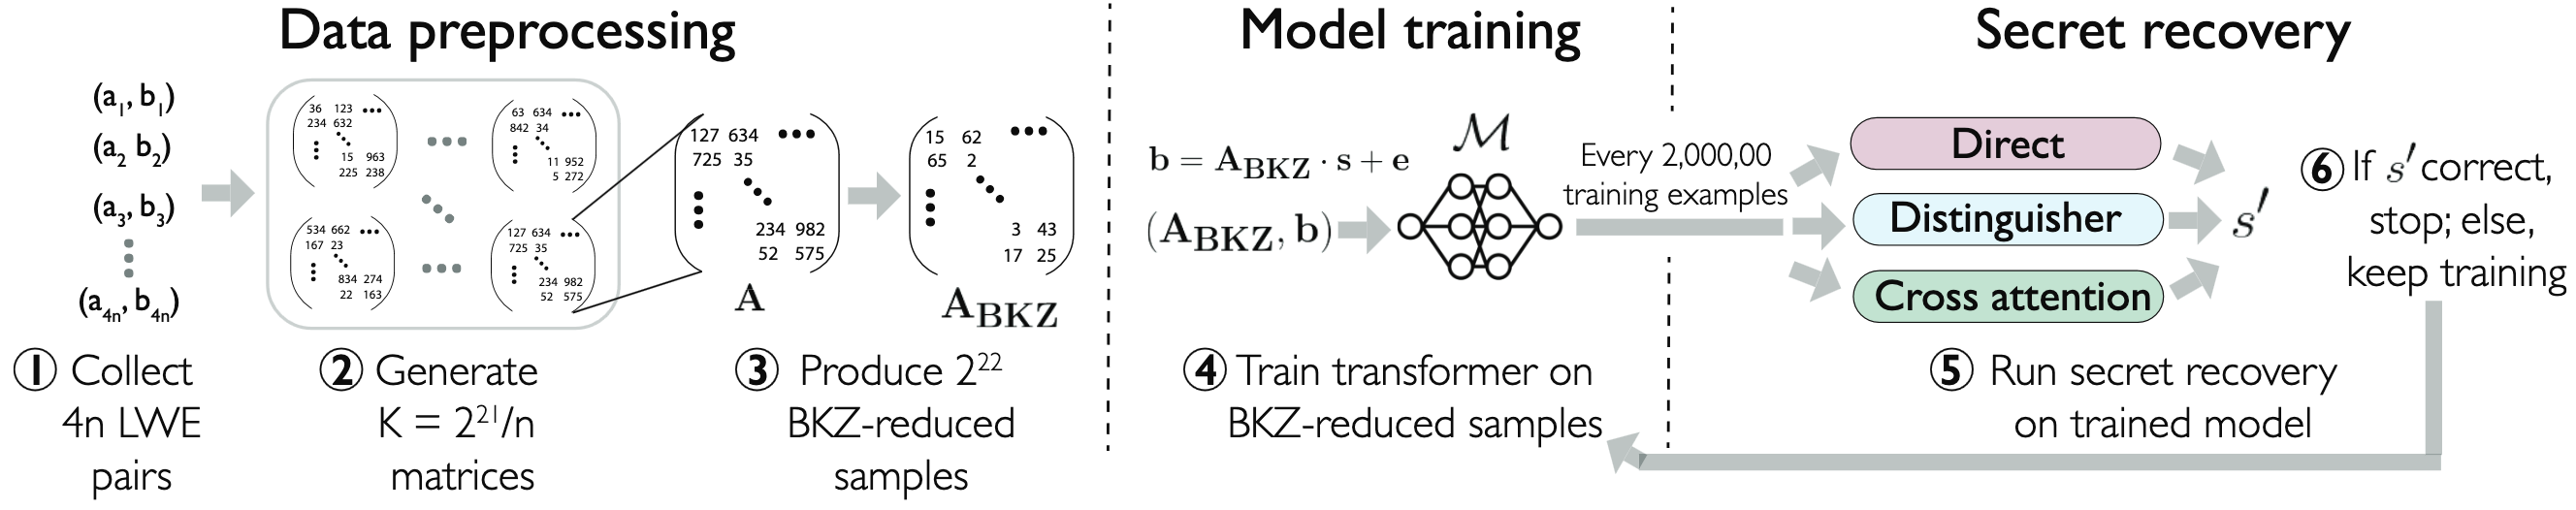
\includegraphics[width=1\textwidth]{Materials/SALSA_PICANTE_Attack_methodology.png}
    \caption{An end-to-end overview of SALSA PICANTE's attack methodology [2]}
    \label{fig:salsa_flowchart}
\end{figure}

\subsubsection{On samples reduction and conformation}
After sampling and recombination, the attack runs a final reduction step to make the LWE samples more amenable to model training. The motivation for this step comes from experimental observations in SALSA. SALSA could only recover binary secrets with low Hamming weights: up to 4 non-zero bits in the secret. However, the SALSA authors observed [3, Table 4] that, if the coordinates of the samples \( a \) used to train the model were bounded by \( \alpha q \), with \( \alpha < 0.6 \), binary secrets with Hamming weights up to 15 could be fully or partially recovered for \( n = 50 \). This result was confirmed for larger dimensions, and different restrictions on \( a \) (e.g. \( a_i \leq \alpha q \) for different \( \alpha \)). Unfortunately, in practical settings, the coordinates of \( a \) are sampled from a uniform distribution over \( \mathbb{Z}_q \), making this technique useless for real-world attacks.

PICANTE turns this observation into a practical attack technique by leveraging existing lattice reduction methods. Such methods reduce the size of the coordinates of LWE samples naturally, yielding the same effect as the SALSA \( \alpha \)-limiting technique. It was found experimentally that reducing LWE samples via these methods before model training allows recovery of secrets with much higher Hamming weights. The reduction technique proceeds as follows.

Given \( n \) LWE samples, stored as the rows of a \( n \times n \) matrix \( A \), and a corresponding vector \( b \) of noisy inner products with a fixed secret \( s \), a matrix \( A' \) can be created with smaller entries than \( A \) by applying standard basis-reduction algorithms like LLL and BKZ to \( \Lambda \), the \( n \)-dimensional lattice defined by the rows of \( A \). In PICANTE, BKZ is run (from the \texttt{fplll} package) on the matrix:
\[
\begin{bmatrix}
\omega \cdot I_n & A_{n \times n} \\
0 & q \cdot I_n
\end{bmatrix},
\]
with \( \omega \in \mathbb{Z} \) as an error penalization parameter, discussed below. Since the BKZ reduction is a change of basis, it is a linear transformation, which can be represented as \( \begin{bmatrix} R_{2n \times n} & C_{2n \times n} \end{bmatrix} \). The BKZ reduction can be written as a matrix multiplication:
\[
\begin{bmatrix} R_{2n \times n} & C_{2n \times n} \end{bmatrix}
\begin{bmatrix}
\omega \cdot I_n & A_{n \times n} \\
0 & q \cdot I_n
\end{bmatrix}
= \begin{bmatrix}
\omega \cdot R & R A + q C
\end{bmatrix},
\]
with matrices \( R \) and \( C \) chosen so that \( \begin{bmatrix} \omega \cdot R & R A + q C \end{bmatrix} \) has \( 2n \) rows with small norms. The matrix \( q C \) adds an integer multiple of \( q \) to each entry in \( R A \), so that all entries are in the range \( (-q/2, q/2] \).

Applying the linear transformation \( R \) to \( b \), a new LWE instance \( (R A, R b) \) is created with the same secret \( s \) and smaller coordinates \( R A \) but a different error distribution. Let \( e = b - A \cdot s \) be the initial LWE error. After reduction, the error becomes \( e' = R b - (R A) \cdot s = R (b - A \cdot s) = R e \). Thus, as \( R \) entries grow, LWE error is amplified. All computations are performed mod \( q \).

Error amplification can be controlled by the error penalization parameter \( \omega \). Recall that BKZ computes \( R \) and \( C \) so that the norms of the rows of \( \begin{bmatrix} \omega \cdot R & R A + q C \end{bmatrix} \) are small. A large \( \omega \) encourages small entries in the rows of \( R \) but hinders the norm reduction of \( R A + q C \), and therefore limits the reduction of \( A \) coordinates. The choice of \( \omega \) controls a trade-off between the amount of reduction of \( a \) that can be achieved, and the amount of additional noise which gets injected in the transformed samples. In practice, \( \omega = 15 \) is set.

When more than \( n \) pairs are available (e.g. the million of pairs produced by Step 1.2), they are divided into batches of \( n \) and processed as above. Thus, \( n \) LWE pairs are transformed into a matrix \( R A \) with \( 2n \) rows, which produces \( \approx 2n \) reduced LWE samples (for \( n \geq 256 \), about 1\% zero rows were observed; this fraction is larger for smaller \( n \)).

\textbf{Note on reduction algorithm choice.} It was experimented with two standard basis-reduction algorithms: LLL and BKZ. Note that the objective is not to find the shortest vector in the lattice defined by \( A \) (the traditional goal of LLL/BKZ), but to transform \( A \) into a matrix with smaller coefficients. Experimentally, it was found that BKZ with small block size (\( \beta = 16 - 20 \)) achieves better reduction than LLL. BKZ speed-ups, such as BKZ2.0, do not seem to result in improved reduction. For BKZ, the block sizes needed to achieve reduction in PICANTE are significantly smaller than the block sizes that would be required to perform a lattice-reduction attack on problems of the same dimensions.

\subsection{Utilized Model and Training}

\subsubsection{Encoding LWE pairs}

Prior to training, \textsc{Picante} encodes the LWE samples (i.e., \( (a, b) \) pairs) as sequences of tokens that the transformer can process. After encoding, the integer coordinates of \( a \) and \( b \) are represented as two digit numbers in base \( B \) (with \( B \approx \sqrt{q} \)). 

Experiments with different values of \( B \) suggest that large values of \( B \), which limit the most significant digit of \( a_i \) and \( b_i \) to a small number of values (i.e. \( B \approx q/k \) with \( k \) small), allow for better performance. In these experiments, \( B = \lfloor q/k \rfloor \) with \( k = 2 \cdot \lfloor n/100 \rfloor + 2 \).

This creates a problem for large dimensions. The large values of \( q \) and \( B \) (for \( n \ge 20 \) we have \( q > 100,000 \) and \( B > 16,600 \)) result in large token vocabularies, which are difficult to learn for a transformer trained on 4 million LWE pairs only. To mitigate this, the lowest digits of \( a \) and \( b \) are encoded into \( B/r \) buckets of size \( r \) (i.e. integer divide them by \( r \)). 

The value \( r \) is chosen so that the overall vocabulary size \( B/r < 10,000 \) (see Table 2). The use of buckets helps train models for large \( n \) but also causes a loss of precision in the values of \( a \) and \( b \). The impact on performance is limited, because the low bits of \( a \) and \( b \) that are rounded off by buckets are those most corrupted by LWE error.

\begin{table}[h]
    \centering
    \begin{tabular}{|c|c|c|c|c|c|c|c|}
        \hline
        $n$ & $q$ & $\log_2 q$ & $\delta$ & $\beta$ & base & $r$ \\
        \hline
        80 & 113 & 7 & 0.99 & 20 & 29 & 1 \\
        150 & 6421 & 13 & 0.99 & 20 & 1071 & 1 \\
        200 & 130769 & 17 & 0.99 & 20 & 21795 & $2^2$ \\
        256 & 6139999 & 23 & 0.96 & 16 & 767500 & $2^7$ \\
        300 & 94056013 & 27 & 0.96 & 16 & 11757002 & $2^{11}$ \\
        350 & 3831165139 & 32 & 0.96 & 14 & 383116514 & $2^{16}$ \\
        \hline
    \end{tabular}
    \caption{Picante parameters. $n$: dimension, $q$: modulus, $\delta$: delta-LLL (BKZ), $\beta$: block-size (BKZ), base: encoding base, $r$: bucket size for encoding.}
    \label{tab:picante_parameters}
\end{table}

\subsubsection{Model Architecture}

As noted previously, \textsc{Picante} uses a transformer model architecture. This architecture, summarized in Figure 2, is strongly inspired by \textsc{Salsa} [3]. Following the proposed, it utilizes a sequence-to-sequence [5] model composed of two transformer stacks - an encoder and a decoder - connected by a cross-attention mechanism. 

The encoder processes the input sequence, the coordinates of $\mathbf{a}$, represented as sequences of digits. The discrete input tokens are first projected over a high-dimensional space (we use dimension $d = 1024$) by a Linear Embedding Layer with trainable weights (i.e. embedding is learned during training). The resulting sequence is then processed by a single-layer transformer: a self-attention layer with 4 attention heads, and a FCNN with one hidden layer of 4096 neurons.

The decoder is an auto-regressive model. It predicts the next token in the output sequence, given already decoded output and the input sequence processed by the encoder. Initially, the decoder is given a beginning of sequence token (BOS), and predicts $b_1^*$, the first digit of $\mathbf{b}$. It is then fed the sequence BOS, $b_1^*$, and decoding proceeds until the end-of-sequence token (EOS) is output.

Decoder input tokens are encoded as 512-dimensional vectors via a trainable embedding (which also decodes transformer output). The decoder has two layers. First, a shared layer (as in shared-layer), which is iterated through 8 times, feeds layer output back into its input. This recurrent process is controlled by a copy-gate mechanism copy-gate, which decides whether a specific token should be processed by the shared layer or just copied as is, skipping the next iteration. After 8 iterations, the output of the shared layer is fed into a “regular” transformer layer. Finally, a linear layer processes the decoder output and computes the probabilities that any word in the vocabulary is the next token. The largest probability is selected via a softmax function (a differentiable counterpart of the max function).

Decoder layers are connected to the encoder via a cross-attention mechanism with 4 attention heads. In each head, the output of the encoder $E = (E_i)_{i \in N_l}$ (with $l$ the input sequence length) is multiplied by two trainable matrices, $W_K$ and $W_V$, yielding the Keys $K = W_K E$ and Values $V = W_V E$. The 512-dimensional vector to be decoded, $D$, is multiplied by a matrix $W_Q$, yielding the Query $Q = W_Q D$. The $l$ scores are calculated from the query and keys:

\[
\text{scores}(E, D) = \text{Softmax}((W_Q D)(W_K E)^\top).
\]

The scores measure how important each encoder input element is when decoding $D$ (i.e. computing $\mathbf{b}$). The cross-attention value for this head is the dot product of scores and values. The values of different heads are then processed by a final linear layer. Cross-attention scores quantify the relation between input positions and output values. \textsc{Picante} uses them to recover the secret bit by bit.

\begin{figure}[h]
    \centering
    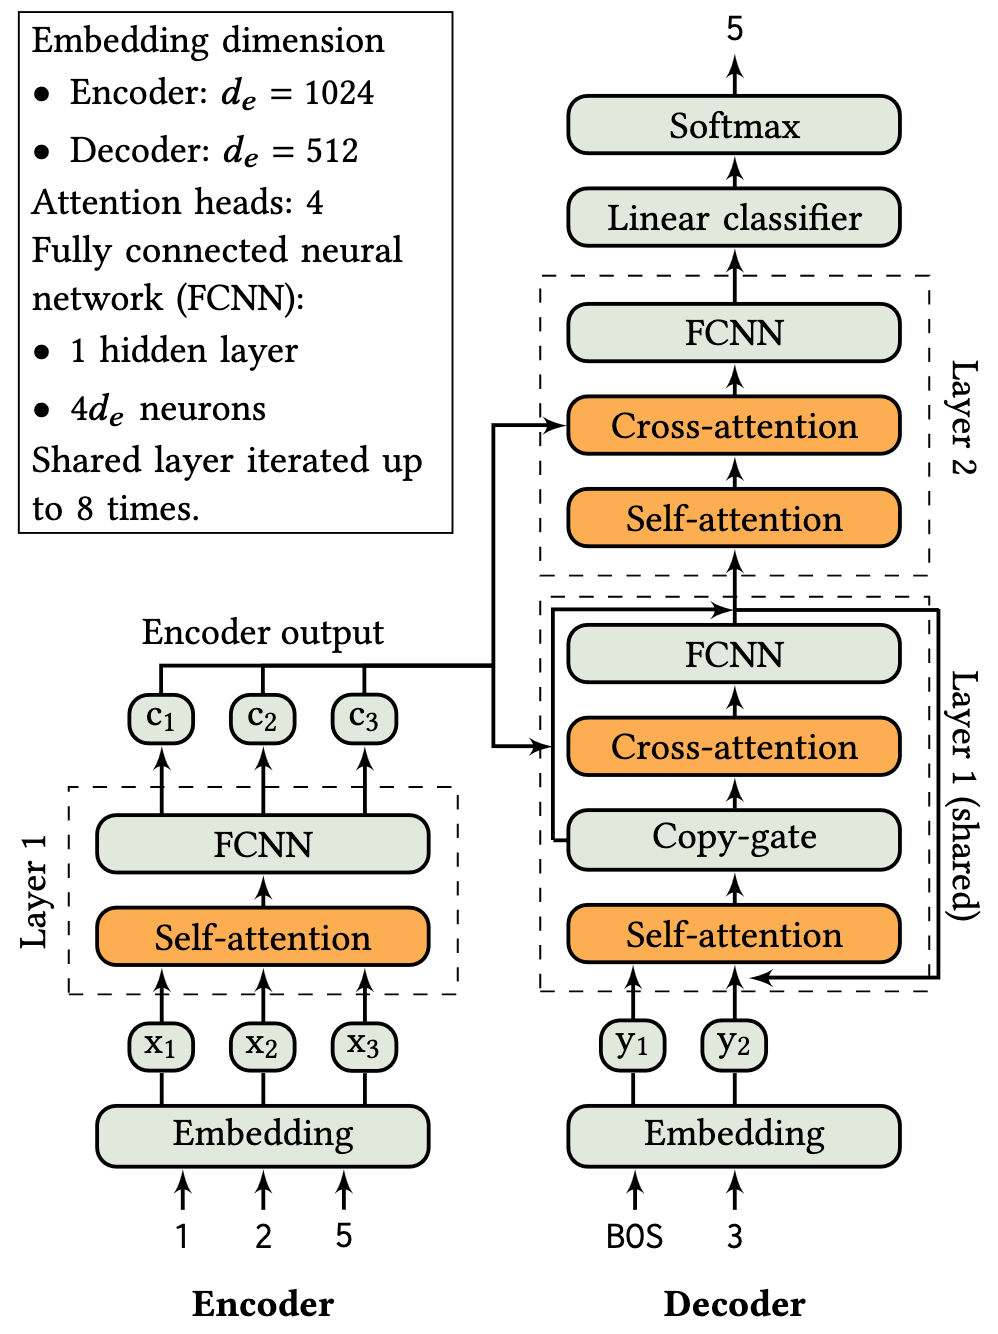
\includegraphics[width=0.42\textwidth]{Materials/PICANTE_Transformer_architecture.png}
    \caption{SALSA PICANTE's transformer architecture [2]}
    \label{fig:salsa_picante_transformer}
\end{figure}

\subsubsection{Model Training}
After encoding the samples, the attacker trains the transformer \( \mathcal{M} \) to predict \( b \) from \( a \). PICANTE frames this as a supervised multi-classification problem, i.e., minimizing the loss:

\begin{equation}
\min_{\theta \in \Theta} \sum_{i=1}^{N} \sum_{j=1}^{K} \sum_{k=1}^{V} 1[y_i[j] = k-1] \frac{e^{\mathcal{M}(x_i)[j,k]}}{\sum_{k'=1}^{V} e^{\mathcal{M}(x_i)[j,k']}}
\end{equation}

where \( \mathcal{M}(x_i) \in \mathbb{R}^{K \times V} \) are model logits evaluated at \( x_i \), \( \theta \in \Theta \) are the model parameters, \( N \) the training sample size, \( K = 2 \) the output sequence length and \( V = B/r \) the vocabulary size.

Solving (1) requires minimizing the cross entropy between model predictions \( \mathcal{M}(a) \) and the ground truth \( b \), over all tokens in the output sequence. Alternatively, one could define this as a regression problem, but it is believed that classification is better adapted to the modular case. Prior works confirm that reformulating regression as classification leads to state-of-the-art performance.

Training proceeds via batches of \( n_b = 128 \) examples. The cross-entropy loss \( \mathcal{L}(\mathcal{M}, a, b) \) is computed over all batch examples, and gradients \( \nabla \mathcal{L} \) are calculated with respect to the model parameters (via back-propagation). Model parameters are then updated using the Adam optimizer, by \( \nabla \mathcal{L} \). The learning rate, \( l \), is set to \( 10^{-5} \), except during the first 1000 optimizer steps, where it is increased linearly from \( 10^{-8} \) to \( 10^{-5} \). Every 2 million examples (an epoch), model performance is evaluated on a held-out sample, and PICANTE attempts to recover the secret. If it fails, another epoch begins.

\subsection{Secret Recovery}

After every training epoch, PICANTE attempts secret recovery. The intuition behind secret recovery is that if a model \(\mathcal{M}\) can predict \(b\) from \(a\) with higher-than-chance accuracy, then \(\mathcal{M}\) must somehow "know" the secret key \(s\), and we can recover \(s\) from \(\mathcal{M}\). SALSA PICANTE uses 3 methods—cross attention, direct recovery, and distinguisher—for recovery. These can be combined for greater accuracy.

In this section, it is assumed that the attacker knows the Hamming weight \(h\) of the secret to be recovered. This is the only part of the attack where this assumption is made. If \(h\) is not known, then secret recovery is run for increasing values of \(h\) until the secret is found.

\subsubsection{Cross-Attention}
In this novel recovery method, PICANTE guesses the secret from the parameters of \(\mathcal{M}\) by leveraging the cross-attention scores of the first decoder layer. Intuitively, the cross-attention score measures the relevance of input tokens (i.e., coordinates of \(a\)) for the computation of \(b\). Since \(b = a \cdot s + e\), the coordinates of \(a\) that correspond to the 0 bits of \(s\) have no impact on \(b\). On the other hand, the coordinates associated with the 1 bits in \(s\) have an impact proportional to their value. Therefore, high cross-attention scores should be found for the input positions that correspond to 1s in the secret.

To run this method, PICANTE evaluates the trained transformer on a test set of 10,000 reduced LWE samples and sums the cross-attention scores of all heads. Since \(a\) has \(n\) coordinates encoded on 2 tokens, this produces a \(2n\)-dimensional vector, from which the odd positions are kept (i.e., the high digits of \(a\) coordinates), generating an \(n\)-dimensional score vector \(V\). A secret guess \(s'\) is then produced by setting the \(h\) largest coordinates of \(V\) to one, and the rest to 0.

\subsubsection{Direct Recovery}
PICANTE uses the same direct recovery method as SALSA. This technique leverages trained transformers’ ability to generalize on inputs not seen during training. The trained model is evaluated on special vectors \(a\) with one non-zero coordinate: \(a = K e_i\) with \(e_i\) the \(i\)-th standard basis vector and \(K \in \mathbb{Z}_q\). For these vectors, since \(b = a \cdot s + e\), and \(e\) is small, \(b \approx 0\) if the \(i\)-th bit in the secret \(s_i = 0\), and \(b \approx K\) if \(s_i = 1\) (see [3] for details). In practice, different \(K_j\) are chosen, and the transformer is run on \(K_j \cdot e_i\) for \(i = 1, \ldots, n\), identifying potential 1-bits in the secret as above and producing a secret guess for each \(K_j\).

To obtain a score for each bit to be used in combination methods, for each index \(i\), we sum the resulting values of \(\mathcal{M}(K_j \cdot e_i)\) (or, equivalently, take the mean). We then guess the secret \(s'\) by assuming that the \(h\) largest coordinates are 1 and the rest are 0.

\subsubsection{Distinguisher}
\textit{Picante}'s version of distinguisher recovery improves upon that of \textit{Salsa}. The general idea is that if the i-th bit of the secret \( s_i = 0 \) and \( e_i \) is the i-th standard basis vector, then the model should predict close values for \( a \) and \( a + K \cdot e_i \). \textit{Salsa}'s distinguisher took a LWE sample \( (a, b) \) and compared \( b \) with the model prediction \( b' = \mathcal{M}(a + K \cdot e_i) \) for some random \( K \in \mathbb{Z}_q \). This presupposed relatively high model accuracy, i.e. \( \mathcal{M}(a) \approx b \), which rarely happens in practice. In \textit{Picante}, \( b' = \mathcal{M}(a + K \cdot e_i) \) is compared to \( \mathcal{M}(a) \) instead of to \( b \). The rest of the method is unchanged, other than implementation improvements. The secret is guessed by setting the \( h \) highest-scoring secret bits to 1, and the rest to 0.

This improved method has two benefits. First it exploits trained model consistency without requiring prediction accuracy. In practice, this means recovery can happen earlier during training, when model prediction accuracy is low. Second, it does not need additional LWE samples \( (a, b) \) (as was the case in \textit{Salsa}), and can be run from randomly generated \( a \). This reduces the number of LWE samples necessary for the attack.

This recovery method relies on a large number of model inferences, which can make it very slow for large dimension. To increase its speed, the same \( a \) is used across all secret bits \( s_i \), halving the number of inferences relative to those required in \textit{Salsa}.

\subsubsection{Combined secret recovery}
Each recovery method outputs a score for every bit in the secret. The secret guess is computed by setting the \( h \) bits with the largest scores to 1 (and the other bits to 0). By combining the scores from different methods, additional techniques are created, which can sometimes recover secrets when individual methods fail. The combined methods are as follows:
\begin{itemize}
    \item \textbf{Aggregated rank.} The bit scores produced by each method are sorted from largest to smallest, and replaced by their rank. The \( h \) bits with the highest ranks (Highest Rank) or highest summed ranks (Sum Rank) are set to 1.
    \item \textbf{Aggregated normalized scores.} The bit scores produced by each method are normalized to \([0, 1]\). The \( h \) bits with the maximum normalized scores (Max Normalized) or the highest sum of normalized scores (Sum Normalized) are set to 1.
\end{itemize}

These combination rules essentially amount to setting secret bits to 1 for bit positions where all, some, or any of the secret recovery methods have a high score. Aggregated scores from all subsets of the secret recovery methods are used. Other combination rules could be considered. These mixing techniques are cheap to implement, because they do not require additional model inferences.

\textbf{Checking correctness.} Recovery methods make guesses \( s' \) about the (unknown) secret \( s \). The test for whether \( s' = s \) was introduced in \textit{Salsa}. On a test sample of \( N_{test} \) LWE pairs \( (a_i, b_i)_{1 \leq i \leq N_{test}} \), compute \( b_i' = a_i \cdot s' \), and consider the distribution \( r \) of \( r_i = b_i' - b_i \mod q \). If \( s' = s \), then \( r \approx e \), the LWE error, with standard deviation \( \sigma \). If \( s' \neq s \), then \( r \) will be approximately uniformly distributed over \( \mathbb{Z}_q \), with standard deviation \( \sigma' = q / \sqrt{12} \). By estimating \( \sigma' \) on a large set of samples, \( s' = s \) can be verified to any confidence level.

This test can be performed on the original set of LWE samples collected by the attacker, e.g. with \( N_{test} = m = 4n \). In §A.2 the authors statistically analyze this verification technique and demonstrate that this sample size is sufficient for all lattice dimensions \( n \geq 80 \).

\subsection{Summary on Attack Methodology}

This section provides an overview of the SALSA PICANTE attack methodology on the LWE problem, detailing the enhancements over the original SALSA attack, which now is divided into three main stages provided below.

\subsubsection{Data Preprocessing}

\begin{itemize}
    \item \textbf{Collect LWE Samples}: The PICANTE attack begins by collecting \(4n\) LWE pairs \((A, b)\) with fixed parameters. This is a significant reduction from the 4 million pairs assumed in the original SALSA attack.
    \item \textbf{Recombine to Expand LWE Sample Set}: Using TinyLWE, the collected samples are expanded to produce a large set of 4 million samples. Subsampling is used instead of linear combinations to avoid amplifying the LWE error.
    \item \textbf{Reduce Samples}: LWE samples are reduced using lattice reduction methods like LLL and BKZ to make them suitable for model training. This reduction allows recovery of secrets with higher Hamming weights.
\end{itemize}

\subsubsection{Model Training}

\begin{itemize}
    \item \textbf{Encoding LWE Pairs}: LWE pairs \((a, b)\) are encoded as sequences of tokens. The integer coordinates are represented as two-digit numbers in base \(B\). Bucketing is used to keep the vocabulary size manageable.
    \item \textbf{Model Architecture}: PICANTE uses a sequence-to-sequence transformer model with an encoder-decoder structure. The encoder processes the input sequences into a high-dimensional space, while the decoder predicts the output sequence. Cross-attention mechanisms connect the encoder and decoder layers.
    \item \textbf{Model Training}: The model is trained to predict \(b\) from \(a\) as a supervised multi-classification problem. The cross-entropy loss function is minimized using the Adam optimizer.
\end{itemize}

\subsubsection{Secret Recovery}

\begin{itemize}
    \item \textbf{Cross-Attention}: This method evaluates the trained transformer's attention scores to guess the secret from reduced LWE samples.
    \item \textbf{Direct Recovery}: Similar to the original SALSA, it leverages the transformer's ability to generalize on special vectors \(a\) with one non-zero coordinate.
    \item \textbf{Distinguisher}: An improved version of the SALSA distinguisher that predicts close values for \(a\) and \(a + K \cdot e_i\). This method reduces the number of required LWE samples by using randomly generated \(a\).
    \item \textbf{Combined Secret Recovery}: Combines scores from different methods (aggregated rank, aggregated normalized scores) to recover the secret more accurately.
    \item \textbf{Checking Correctness}: Verifies the guessed secret against the actual secret using a statistical analysis of the verification technique.
\end{itemize}

\section{SALSA PICANTE'S PERFORMANCE}
\label{sec:salsa_picante_performance}

We now evaluate Picante's performance over a variety of parameter settings for lattice dimension, modulus size, Hamming weight, and number of samples. All Picante experiments are based on the following choices, with the exact parameters used in our experiments listed in Table 2. Other details are in \S4.

\subsection{Experimental settings}

\begin{itemize}
    \item For each \(n\), the modulus \(q\) is selected after considering the security of LWE with small secret, [2, ref 12]. Next, set \(q\) such that \(\log_2 q\) is smaller than the smallest successful lattice-reduction attack reported there (see Table 2). A smaller \(q\) makes attacks more difficult.
    \item The error in the original LWE samples is sampled from a discrete Gaussian distribution, centered at 0, and with \(\sigma = 3\), a common choice when LWE is used in homomorphic encryption [2, ref 2,3].
    \item Consider binary secrets with sparsity \(h/n \approx 10\%\) or larger. For each \(n\) where evaluate Picante, results for seven different Hamming weights \(h \approx n/10\) to confirm repeatability, are shown.
    \item The attack starts with a set of \(4n\) randomly generated samples \((a, b)\) with fixed \(n\), \(q\), sparse binary \(s\), and \(\sigma\).
    \item For the BKZ reduction step (Picante stage 3), used \(\omega = 15\) as the error penalization parameter for all \(n\). Block size and the LLL parameter \(\delta\) in \textit{fplll} are set to 20 and 0.99 for all \(n \leq 200\). To keep preprocessing times reasonable, decrease these values for \(n = 256, 300\) and \(350\) (Table 3).
    \item For each \(n\) and \(q\), perform the preprocessing step on random matrices \(A\) once and use that reduced data for experiments with different secrets.
\end{itemize}

\begin{table}[h]
    \centering
    \begin{tabular}{|c|c|c|c|c|c|c|}
        \hline
        \textbf{\(n\)} & \textbf{\(\log_2 q\)} & \textbf{\(\delta\)} & \textbf{\(\beta\)} & \textbf{\(\text{std}(A)/\text{std}(A_{rand})\)} & \textbf{\(\text{max } h\)} \\
        \hline
        80 & 7 & 0.99 & 20 & 0.78 & 9 \\
        150 & 13 & 0.99 & 20 & 0.53 & 13 \\
        200 & 17 & 0.99 & 20 & 0.40 & 22 \\
        256 & 23 & 0.96 & 20 & 0.33 & 31 \\
        300 & 27 & 0.96 & 16 & 0.32 & 33 \\
        350 & 32 & 0.96 & 14 & 0.25 & 60 \\
        \hline
    \end{tabular}
    \caption{Preprocessing parameters for BKZ in \textit{fplll} for \textsc{Picante}'s best secret recoveries. \(\beta\) : block size, \(\delta\) : LLL\_DELTA.}
\end{table}

\subsection{Overall Performance}

A summary of PICANTE’s results is shown in Table 3, which records PICANTE’s success for various dimensions \( n \), modulus \( q \), and Hamming weight \( h \). Multiple experiments are run for each parameter setting, and the number of successes/attempts, as well as the model training epochs at which successful secret recoveries occurred, are reported. For example, in dimension \( n = 350 \), a secret with \( h = 60 \) was recovered in one out of five trials (each trial has a different secret). In that case, the recovery happened in training epoch 38.

\subsubsection{Effect of dimension \( n \)}

For dimensions up to 300, PICANTE consistently recovers LWE secrets with sparsity \( h/n \approx 10\% \), a significant improvement over SALSA. For \( n = 350 \), PICANTE can recover secrets with Hamming weight \( h = 60 \), sparsity \( \approx 17\% \). This improved performance is due to the preprocessing parameters used for \( n = 350 \). This suggests that harder LWE problems, with dimension \( n = 350 \) but smaller \( q \), could be solved with this architecture for \( h \approx 0.1n \).

For all dimensions, PICANTE succeeds for smaller values of the modulus \( q \) than those for which the concrete, classical lattice attacks in \cite{12} can recover secrets with BKZ blocksize roughly 40. In the experiments, a fixed \( q \) for each dimension is used to avoid running the costly preprocessing step multiple times. Evaluating performance at varying \( q \) for a fixed \( n \) is important future work.

\subsubsection{Effect of Hamming weight \( h \)}

For each dimension \( n \), PICANTE is evaluated on secrets with a range of Hamming weights. For each \( n \), there is a “cutoff” Hamming weight, above which PICANTE did not successfully recover the secret in these runs. This is expected, because increasing Hamming weight makes the problem more difficult. Figure 3 presents the cutoff value in bold, along with the number of successfully recovered secrets for each Hamming weight.

\begin{figure}[h]
    \centering
    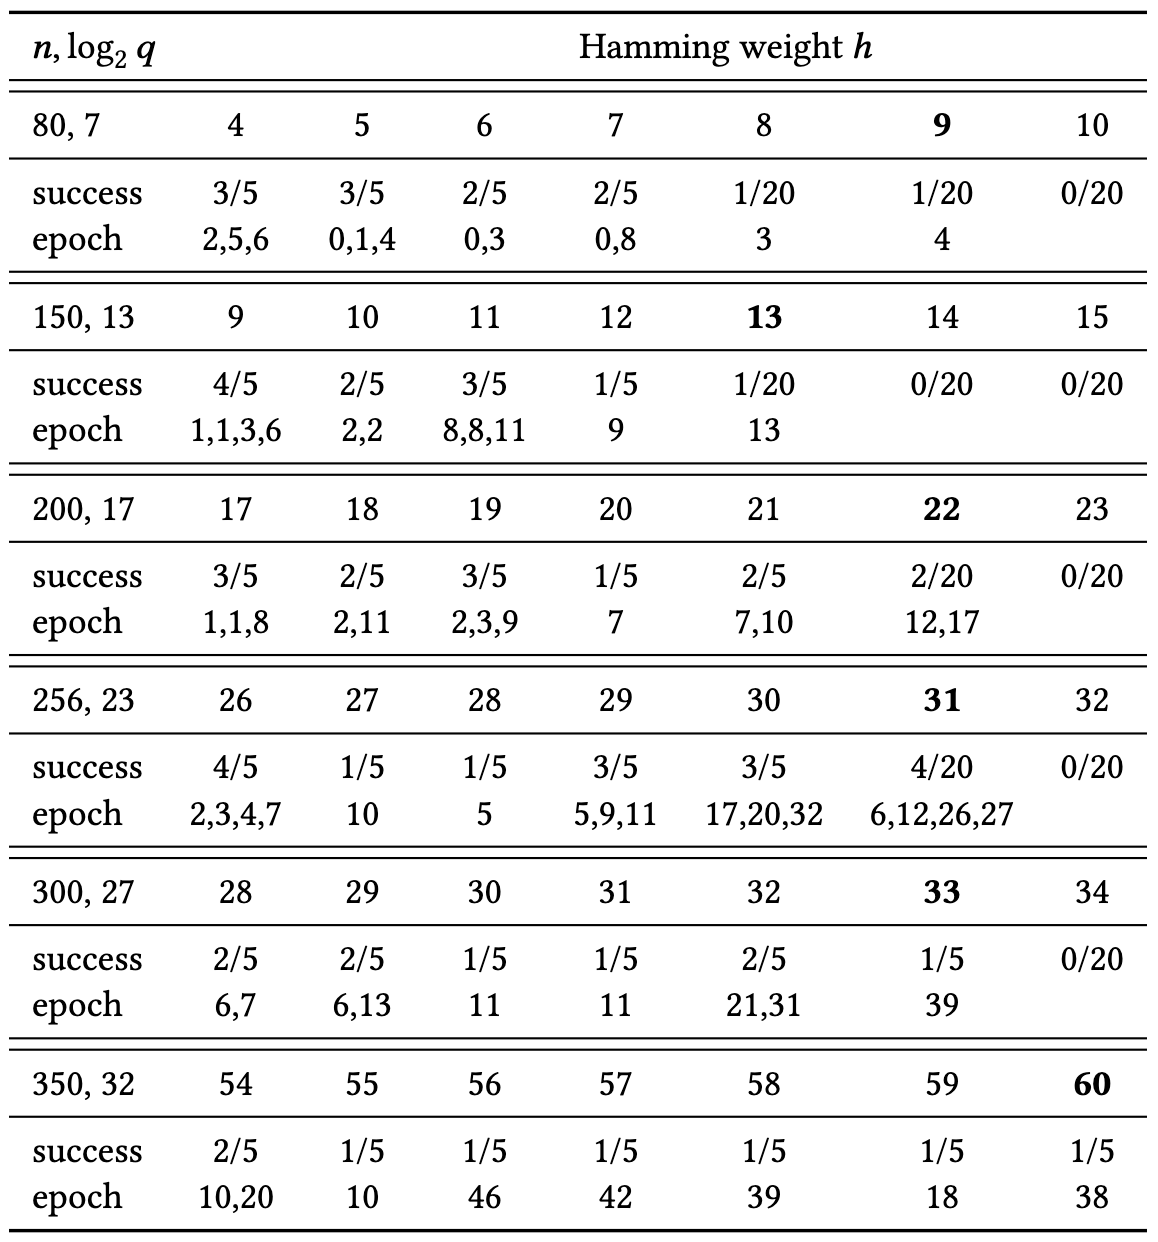
\includegraphics[width=0.6\textwidth]{Materials/Picante_performance.png}
    \caption{Success rates and number of epochs. Highest recovered Hamming weight for each dimension \( n \) is in \textbf{bold}}
    \label{fig:picante_performance}
\end{figure}

\subsubsection{Effect of dimension \( n \)}

For dimensions up to 300, PICANTE consistently recovers LWE secrets with sparsity \( h/n \approx 10\% \), a significant improvement over SALSA. For \( n = 350 \), PICANTE can recover secrets with Hamming weight \( h = 60 \), sparsity \( \approx 17\% \). This improved performance is due to the preprocessing parameters used for \( n = 350 \). This suggests that harder LWE problems, with dimension \( n = 350 \) but smaller \( q \), could be solved with this architecture for \( h \approx 0.1n \).

For all dimensions, PICANTE succeeds for smaller values of the modulus \( q \) than those for which the concrete, classical lattice attacks in \cite{12} can recover secrets with BKZ blocksize roughly 40. In the experiments, a fixed \( q \) for each dimension is used to avoid running the costly preprocessing step multiple times. Evaluating performance at varying \( q \) for a fixed \( n \) is important future work.

\subsubsection{Effect of Hamming weight \( h \)}

For each dimension \( n \), PICANTE is evaluated on secrets with a range of Hamming weights. For each \( n \), there is a “cutoff” Hamming weight, above which PICANTE did not successfully recover the secret in these runs. This is expected, because increasing Hamming weight makes the problem more difficult. Figure 3 presents the cutoff value in bold, along with the number of successfully recovered secrets for each Hamming weight.

\begin{figure}[h]
    \centering
    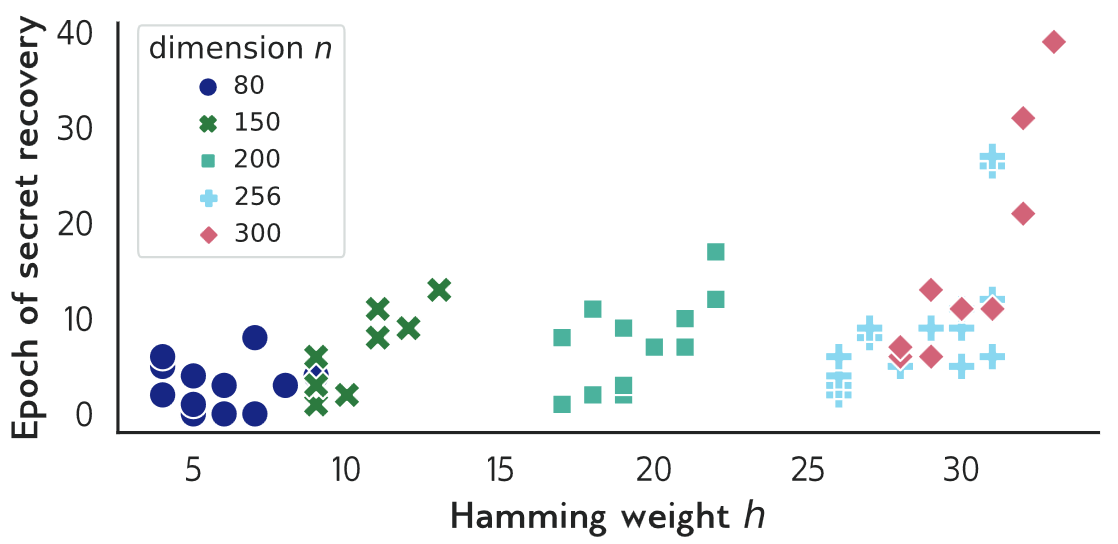
\includegraphics[width=0.45\textwidth]{Materials/Picante_performance_chart.png}
    \caption{N of training epochs before secret recovery for n=[80, 300] on dim and Hamming weights.}
    \label{fig:picante_performance_chart}
\end{figure}

\subsubsection{Required Training Duration}

Figure 4 shows the number of epochs needed for secret recovery for \(80 \leq n \leq 300\) and different values of \(h\). Whereas 66\% of successful secret recoveries occurred during the first 10 epochs, the number of epochs before recovery increases with \(n\) and \(h\). For \(n = 80\), about 75\% of successful experiments succeed by epoch 4. Eight epochs are needed for 75\% of experiments to succeed for \(n = 150\), and 13 epochs for \(n = 200, 256, 300\).

For a given dimension, the number of epochs required for secret recovery varies a lot from one experiment to another. For dimension 256 and Hamming weight 31, different secrets need between 6 and 27 epochs. For dimension 350, a secret with Hamming weight 59 is recovered after 18 epochs, while secrets with \(h = 58\) and 60 need 39 and 38.

It is believed that, for a given secret \(s\), certain distributions of the coordinates of \(a\) help the transformer learn \(s\). The proportion of such points \(a\) in the training sample varies for different secrets, making some harder to recover, and necessitating longer training.

Another explanation for the variations in training length is the random initialization of transformer parameters. For a given secret, running several experiments, with different initializations, may reduce the number of epochs required for recovery.

\subsubsection{Required LWE Sample Size}

PICANTE relies on the TinyLWE subsampling technique introduced in section 3.1 to recover secrets from only \(4n\) initial LWE samples. By comparison, SALSA used 4 million LWE samples. Table 4 compares the performance of PICANTE (using TinyLWE), with an equivalent attack using 2.2 million collected LWE samples, which we call LWE. For both sampling approaches—TinyLWE and LWE—the reduction step described in 3.1.3, is run before performing model training and secret recovery.

\begin{table}[h]
    \centering
    \begin{tabular}{|c|c|c|c|c|c|c|}
        \hline
        \textbf{Dimension} & \textbf{80} & \textbf{150} & \textbf{200} & \textbf{256} & \textbf{300} \\
        \hline
        \textbf{TinyLWE max \( h \)} & 9 & 13 & 22 & 31 & 33 \\
        \textbf{LWE max \( h \)} & 9 & 12 & 21 & 32 & 32 \\
        \hline
    \end{tabular}
    \caption{TinyLWE vs LWE. Values: highest \(h\) recovered for each \(n\).}
\end{table}

%SALSA VERDE
\section{SALSA VERDE Overview}

In this section, we describe the SALSA VERDE attack and relevant parts of its predecessor PICANTE.

\begin{figure}[h]
    \centering
    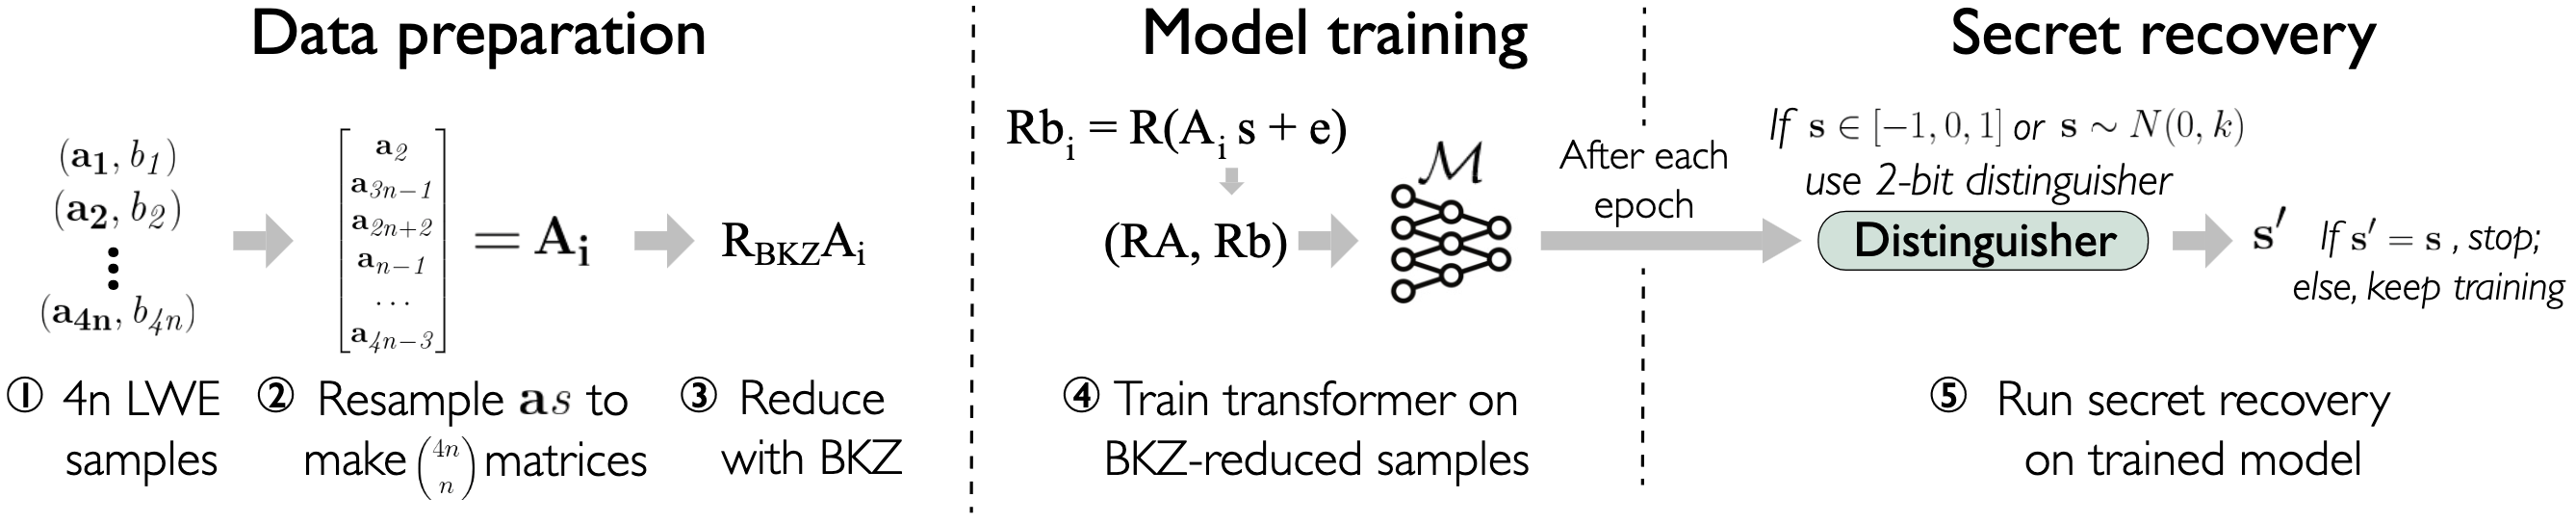
\includegraphics[width=\textwidth]{Materials/SALSA_VERDE_Attack_methodology.png}
    \caption{Overview of VERDE's attack methodology}
\end{figure}

\subsection{High-level overview}
Like PICANTE, VERDE starts with $4n$ LWE samples with the same secret $s$. In practice, this data would be eavesdropped. VERDE then proceeds in three stages: preprocessing, model training, and secret recovery (see Figure 1). The preprocessing stage augments the $4n$ initial $(a, b)$ pairs to 2 million, then runs lattice reduction to yield a training set of 4 million samples with the same secret $s$. The preprocessed data is used to train a transformer to predict $b$ from $a$. After each training epoch (2 million LWE samples), the model is queried to form a secret guess. The attack succeeds if the secret guess is correct, tested via statistical methods without knowledge of the actual secret. Otherwise, the model is trained for another epoch, and secret recovery is run again.

\subsection{Data preprocessing}
VERDE's preprocessing is similar to PICANTE's, with several improvements. First, $n \times n$ matrices $A_i$ are created by sampling without replacement $n$ of the $4n$ original LWE samples. Then, lattice reduction is applied to the matrices $A_i$ to reduce the standard deviation of their entries (initially uniformly distributed over $[0, q]$). This process generates $2n$ preprocessed samples $(a', b')$, with the same secret and is implemented in parallel to create a training set of 4 million samples.

During lattice reduction, PICANTE applies BKZ (as implemented in \texttt{fplll} \cite{27}) to the $2n \times 2n$ matrix:
\[
\Lambda_i = \begin{bmatrix}
\omega \cdot I_n & A_i \\
0 & q \cdot I_n
\end{bmatrix}.
\]
BKZ finds a linear transformation $[R_i, C_i]$ such that the norms of the $2n$ rows of $[R_i, C_i] A_i = [\omega \cdot R_i, R_i A_i + q \cdot C_i]$ are small. Applying $R_i$ to $A_i$ and $b_i$, PICANTE generates $2n$ reduced LWE pairs $(R_i A_i, R_i b_i)$ (modulo $q$). VERDE instead rearranges the rows of $\Lambda_i$ and applies lattice reduction to $A_i'$:
\[
A_i' = \begin{bmatrix}
0 & q \cdot I_n \\
\omega \cdot I_n & A_i
\end{bmatrix}.
\]
This reduces the number of operations needed for lattice reduction and allows BKZ to run with lower floating point precision. These two improvements reduce the operations required for VERDE's preprocessing.

\subsection{Model training}
VERDE trains a transformer model $\mathcal{M}$ to predict $b$ from $a$. The model is trained on the BKZ-reduced samples $(RA, Rb)$, where $Rb_i = R(A_i s + e)$. After each epoch, the model is queried to form a secret guess $s'$. The attack proceeds until the guess is correct or training reaches a predefined number of epochs. 

\subsection{Secret recovery}
VERDE employs a distinguisher approach for secret recovery. If $s \in [-1, 0, 1]$ or $s \sim N(0, k)$, a 2-bit distinguisher is used. The model is queried for each reduced sample $(RA, Rb)$ and a secret guess $s'$ is formed by setting the highest scoring secret bits to 1, and the rest to 0. The attack succeeds if $s' = s$, else the model continues training.

In summary, VERDE's attack methodology improves on PICANTE by reducing the computational load of preprocessing and enhancing the secret recovery process with a more effective distinguisher.

\section{SALSA Verde New Approaches and Methodologies}

\subsection{Two-Bit Distinguisher}

\textbf{Concept:} SALSA Verde introduces a two-bit distinguisher, an advanced technique for secret recovery that significantly improves upon the previous single-bit distinguisher used in PICANTE.
\textbf{Application:} The two-bit distinguisher is designed to be effective for recovering secrets that are sparse binary, ternary, or follow a narrow Gaussian distribution. This makes it versatile and suitable for a wider range of cryptographic scenarios.
\textbf{Advantage:} The primary advantage of the two-bit distinguisher is its enhanced capability to fully recover these types of secrets. By considering two bits at a time, the distinguisher provides a more detailed analysis of the secret structure, leading to improved recovery rates.

\vspace{3mm}

\textbf{Implementation Details:}

\begin{itemize}
    \item \textbf{Input Data:} The two-bit distinguisher operates on reduced LWE samples $(RA, Rb)$, where $Rb = R(A \cdot s + e)$, and $s$ is the secret to be recovered.
    \item \textbf{Recovery Process:} The process involves evaluating the model on each reduced sample and forming a secret guess $s'$ based on the scores. The distinguishing process leverages statistical methods to determine the likelihood of each bit being part of the secret.
    \item \textbf{Statistical Evaluation:} The distinguishing process evaluates the scores of pairs of bits to decide their values. If $s \in \{-1, 0, 1\}$ or follows a Gaussian distribution $N(0, k)$, the two-bit distinguisher is particularly effective.
    \item \textbf{Enhanced Accuracy:} By considering two bits simultaneously, the method increases the accuracy of the secret recovery, reducing the chances of errors compared to the single-bit approach.
\end{itemize}

\subsection{Improved Data Preprocessing}

\textbf{Concept:} SALSA Verde introduces a significantly improved data preprocessing methodology. This involves the creation of \( n \times n \) matrices and the application of advanced lattice reduction techniques, which together make the preprocessing stage more efficient and effective.

\vspace{3mm}

\textbf{Redesigned Matrices:}

\begin{itemize}
    \item \textbf{Creation of Matrices:} SALSA Verde generates \( n \times n \) matrices \( A_i \) by sampling without replacement from the original LWE samples. This technique ensures that each matrix \( A_i \) is a unique permutation of the original samples, which helps in reducing redundancy and enhancing the overall effectiveness of the attack.
    \item \textbf{Sampling Without Replacement:} This method ensures that the same sample is not reused within the same matrix, which helps in maintaining the diversity of the data used for training.
\end{itemize}

\textbf{Lattice Reduction:}

\begin{itemize}
    \item \textbf{Application of Lattice Reduction:} SALSA Verde applies lattice reduction techniques to the matrices \( A_i \) to reduce the standard deviation of their entries. This step is crucial as it transforms the matrices in a way that makes the subsequent steps of the attack more efficient.
    \item \textbf{Re-ordered Matrix:} By rearranging the rows of the matrices, the lattice reduction is performed on a more optimized version of the original data. This reordering is designed to achieve lower floating-point precision and better reduction results.
\end{itemize}

\textbf{Efficiency:}

\begin{itemize}
    \item \textbf{Speed and Effectiveness:} The preprocessing in SALSA Verde is forty times faster and 20\% more effective than in PICANTE. This substantial improvement in speed and effectiveness allows SALSA Verde to handle larger dimensions (up to 512) and smaller moduli (down to \( \log_2 q = 12 \) for \( n = 256 \)).
    \item \textbf{Handling Larger Dimensions:} With these improvements, SALSA Verde can manage much larger dimensions and smaller moduli than PICANTE, significantly enhancing its applicability and performance in various cryptographic contexts.
\end{itemize}

\subsection{Enhanced Lattice Reduction Techniques}

\textbf{Concept:} SALSA Verde employs enhanced lattice reduction techniques that improve the efficiency and effectiveness of the preprocessing stage. These techniques include reordered lattice reduction, interleaved algorithms, and adaptive block size and precision adjustments.

\vspace{3mm}

\textbf{Reordered Lattice Reduction:}

\begin{itemize}
    \item \textbf{Optimization by Reordering:} SALSA Verde reorders the rows of the lattice matrix \( \Lambda_i \) to optimize the reduction process. This reordering is based on a strategy that reduces the computational complexity and enhances the quality of the reduced lattice.
    \item \textbf{Implementation:} By carefully reordering the rows, the lattice reduction algorithms can work more effectively, leading to faster convergence and better results in the subsequent stages of the attack.
\end{itemize}

\textbf{Interleaved Algorithms:}

\begin{itemize}
    \item \textbf{Use of BKZ 2.0:} SALSA Verde utilizes the BKZ 2.0 algorithm, which is known for its efficiency and effectiveness in lattice reduction. BKZ 2.0 improves upon the traditional BKZ algorithm by incorporating additional optimization techniques.
    \item \textbf{Efficient Reduction Technique:} Alongside BKZ 2.0, SALSA Verde integrates an efficient reduction technique that works in tandem with BKZ 2.0. This interleaving of two algorithms reduces the computational burden and improves the overall reduction process.
    \item \textbf{Benefit:} The combination of these two algorithms allows for a more robust reduction process, leading to better performance and faster preprocessing times.
\end{itemize}

\textbf{Adaptive Blocksize and Precision:}

\begin{itemize}
    \item \textbf{Dynamic Adjustments:} During the reduction process, SALSA Verde adjusts the block size and precision dynamically. This adaptive approach ensures that the reduction process remains efficient while maintaining high quality.
    \item \textbf{Preprocessing Time:} By adjusting these parameters on-the-fly, SALSA Verde significantly cuts down on preprocessing time. The ability to fine-tune block size and precision allows for optimal performance under varying conditions.
    \item \textbf{Quality Improvement:} The dynamic adjustments not only speed up the reduction process but also enhance the quality of the reduced lattice. This improvement is crucial for the success of the subsequent stages of the attack.
\end{itemize}

\subsection{Secret Recovery Techniques}

\textbf{Concept:} SALSA Verde focuses on a streamlined and optimized approach for secret recovery, utilizing an enhanced distinguisher method and testing with preprocessed vectors to improve generalization and performance.

\vspace{3mm}

\textbf{Exclusive Use of Distinguisher:}

\begin{itemize}
    \item \textbf{Methodology Shift:} Unlike PICANTE, which utilized three different methods (direct recovery, cross-attention, and distinguisher), SALSA Verde exclusively employs an enhanced distinguisher method. This method is specifically optimized for the preprocessed data, making the recovery process more efficient.
    \item \textbf{Enhanced Distinguisher:} The enhanced distinguisher in SALSA Verde leverages the improvements made in data preprocessing and lattice reduction. It is designed to work more effectively with the high-quality preprocessed data, leading to better recovery rates.
\end{itemize}

\textbf{Testing with Preprocessed Vectors:}

\begin{itemize}
    \item \textbf{Preprocessed Vector Usage:} SALSA Verde improves upon the random vector testing approach by using a held-out subset of preprocessed vectors. This approach ensures that the testing phase benefits from the same high-quality data used during training.
    \item \textbf{Model Generalization:} By testing on preprocessed vectors, the model's ability to generalize is significantly enhanced. This results in a more robust performance during the secret recovery phase.
    \item \textbf{Recovery Performance:} The use of preprocessed vectors also improves the overall recovery performance, as the model is evaluated on data that is more representative of the training set, leading to more accurate and reliable secret recovery.
\end{itemize}

\subsection{Transformer Training}

\textbf{Concept:} SALSA Verde builds on the seq2seq transformer architecture used in PICANTE, incorporating several key enhancements to improve training efficiency and effectiveness.

\vspace{3mm}

\textbf{Model Structure:}
\begin{itemize}
    \item \textbf{Seq2seq Transformer Architecture:} SALSA Verde uses a sequence-to-sequence (seq2seq) transformer model, similar to that used in PICANTE. This architecture is well-suited for the task of predicting sequences of \( b \) from sequences of \( a \).
    \item \textbf{Rotary Word Embeddings:} One of the notable enhancements in Verde is the use of rotary word embeddings. These embeddings allow for more effective handling of positional information in the sequences, leading to better performance.
    \item \textbf{Earth Mover’s Distance (EMD) Auxiliary Objective:} Verde also incorporates an earth mover’s distance (EMD) auxiliary objective. This objective helps the model by providing an additional optimization target that aligns the predicted distributions more closely with the true distributions, improving the overall training outcome.
\end{itemize}

\textbf{Training Optimization:}
\begin{itemize}
    \item \textbf{Translation Task Framing:} The model training is framed as a translation task, where sequences representing \( a \) are translated into sequences representing \( b \). This framing is effective in leveraging the capabilities of the transformer architecture.
    \item \textbf{Minimizing Cross-Entropy Loss:} The primary objective during training is to minimize the cross-entropy loss between the predicted sequences and the true sequences. This loss function is well-suited for classification tasks and ensures that the model learns to make accurate predictions.
    \item \textbf{Efficient GPU Training:} The setup allows for efficient training on NVIDIA V100 GPUs. The powerful computational capabilities of these GPUs enable rapid convergence, allowing the model to quickly learn and recover secrets.
\end{itemize}

\subsection{Evaluation and Performance Metrics}

\textbf{Concept:} SALSA Verde emphasizes efficient sample generation and demonstrates its capability to handle larger dimensions and smaller moduli compared to its predecessor, PICANTE.

\vspace{3mm}

\textbf{Reduction in Required Samples:}
\begin{itemize}
    \item \textbf{TinyLWE Subsampling Technique:} SALSA Verde employs the TinyLWE subsampling technique to efficiently generate a large number of training samples from a small initial set. This technique is crucial in scaling the attack to practical settings where obtaining a massive number of initial samples is impractical.
    \item \textbf{Efficient Generation of Training Samples:} By leveraging the TinyLWE method, Verde can produce the required \( 4n \) LWE samples from a significantly smaller base set, thereby reducing the resource requirements for executing the attack.
\end{itemize}

\textbf{High Dimensionality and Small Moduli:}
\begin{itemize}
    \item \textbf{Larger Dimensions:} SALSA Verde demonstrates successful secret recovery for larger dimensions than what was achievable with PICANTE. This capability is attributed to the improved preprocessing and enhanced lattice reduction techniques, which allow the system to manage and process higher-dimensional data effectively.
    \item \textbf{Smaller Moduli:} Verde also operates effectively with smaller moduli, expanding the range of cryptographic parameters that can be targeted. The system's ability to work with log\(_2 q\) as small as 12 for \( n = 256 \) showcases its enhanced flexibility and robustness in cryptographic attacks.
\end{itemize}

\subsection{Theoretical Analysis}

\textbf{Concept:} SALSA Verde incorporates a theoretical framework to understand and predict the success of machine learning (ML)-based LWE attacks, focusing on the relationship between secret recovery success and the parameters involved.

\vspace{3mm}

\textbf{Scaling Laws:}
\begin{itemize}
    \item \textbf{NoMod Framework:} SALSA Verde introduces the NoMod (No Modulus) theoretical framework. This framework is crucial for analyzing and understanding the dynamics of ML-based attacks on LWE. It helps to delineate the conditions under which secret recovery is successful and provides insights into the scalability of such attacks.
    \item \textbf{Dependence on \(\sqrt{h}\):} The NoMod framework highlights that the success of secret recovery depends on the square root of (\(h\)) of the secret. This insight is significant because it provides a quantifiable measure to predict the effectiveness of the attack based on the sparsity of the secret.
    \item \textbf{Mathematical Rationale:} The framework mathematically explains why and how the success rate of ML-based LWE attacks scales with the Hamming weight of the secret. It offers a deeper understanding of the attack's success probability and helps optimize the attack parameters for different scenarios.
\end{itemize}

\section{SALSA Verde's Performance}

This section evaluates SALSA Verde's performance over various parameter settings for lattice dimension, modulus size, Hamming weight, and the number of samples. 

\subsection*{Performance on Small q}

SALSA Verde significantly outperforms PICANTE in recovering binary secrets with smaller modulus \( q \). Table 6 shows the highest recovered \( h \) for dimensions 256 and 350 and different \( q \) for binary, ternary, and Gaussian secrets. Verde succeeds with smaller \( q \), demonstrating its enhanced capabilities.

\begin{table}[h]
    \centering
    \begin{tabular}{|c|c|c|c|c|}
        \hline
        \textbf{\( n, \log_2 q \)} & \textbf{reduction factor} & \textbf{b} & \textbf{t} & \textbf{g} \\
        \hline
        256, 20 & 0.43 & 33 & 24 & 7 \\
        256, 18 & 0.53 & 18 & 19 & 7 \\
        256, 16 & 0.63 & 12 & 12 & 6 \\
        256, 14 & 0.71 & 9 & 9 & 6 \\
        256, 12 & 0.77 & 6 & 6 & 5 \\
        \hline
        350, 27 & 0.38 & 36 & 36 & 10 \\
        350, 21 & 0.61 & 12 & 13 & 5 \\
        \hline
    \end{tabular}
    \caption{Highest \( h \) recovered, \( n = 256, 350 \). Secret distributions are \( b \) = binary, \\ \( t \) = ternary, \( g \) = Gaussian.}
\end{table}

\subsection*{Effect of Dimension and Hamming Weight}

Figure 3 shows the number of epochs needed for secret recovery for \( 80 \leq n \leq 300 \) and different values of \( h \). The success rate decreases as \( h \) increases. Verde's preprocessing factor significantly contributes to its ability to recover secrets for larger dimensions and smaller moduli.

\subsection*{Reduction in Required Samples}

Using the TinyLWE subsampling technique, SALSA Verde efficiently generates large numbers of training samples from a small initial set. This reduction in required samples enables effective scaling to larger dimensions and smaller moduli.

\subsection*{Theoretical Analysis}

The NoMod framework provides a theoretical basis for understanding the success of ML-based LWE attacks. It shows that the success of secret recovery depends on \( \sqrt{h} \) of the secret, providing insights into optimizing attack parameters.

Overall, SALSA Verde's improved preprocessing, enhanced lattice reduction techniques, and advanced recovery methods demonstrate significant advancements over PICANTE, particularly in handling larger dimensions and smaller moduli.


\subsection*{Overview of SALSA PICANTE's Transformer Architecture}

The \textbf{SALSA PICANTE} model is designed using a \textbf{sequence-to-sequence (seq2seq) transformer architecture}. Here's a detailed breakdown of its components and functionalities:

\textbf{1. Embedding Dimension}
\begin{itemize}
    \item \textbf{Encoder}: The embedding dimension is set to \(d_e = 1024\). This allows the encoder to represent the input data in a high-dimensional space, capturing complex patterns and relationships.
    \item \textbf{Decoder}: The embedding dimension for the decoder is \(d_e = 512\). This helps in efficiently transforming the encoded data back to the target sequence.
\end{itemize}

\textbf{2. Attention Mechanism}
\begin{itemize}
    \item The model utilizes \textbf{4 attention heads}. Attention heads are crucial for capturing different aspects of the input sequence, allowing the model to focus on relevant parts of the data during processing.
\end{itemize}

\textbf{3. Fully Connected Neural Network (FCNN)}
\begin{itemize}
    \item The FCNN consists of \textbf{1 hidden layer} with \textbf{\(4d_e\) neurons}. This layer performs complex transformations on the data, enabling the model to learn intricate patterns.
    \item The \textbf{shared layer} in the FCNN can be iterated up to \textbf{8 times}, enhancing the model's ability to refine its understanding of the input data through repeated processing.
\end{itemize}

\textbf{4. Encoder}
\begin{itemize}
    \item \textbf{Input Processing}: The encoder begins by processing the input sequences (\(x_1, x_2, x_3\)). These inputs are initially passed through an \textbf{embedding layer}, which converts the raw input into high-dimensional vectors.
    \item \textbf{Self-Attention Layer}: The embedded inputs then pass through a \textbf{self-attention layer}, where the model weighs the importance of each part of the input sequence relative to others. This helps in understanding the context and relationships within the data.
    \item \textbf{FCNN Layer}: After self-attention, the data is processed by an \textbf{FCNN layer}, which applies nonlinear transformations to capture complex features.
    \item \textbf{Encoder Output}: The processed data, now represented as \(c_1, c_2, c_3\), is passed to the decoder.
\end{itemize}

\textbf{5. Decoder}
\begin{itemize}
    \item \textbf{Sequence Tokens}: The decoder starts with sequence tokens (BOS, \(y_1, y_2\)), which are embeddings of the beginning of the sequence and previously decoded tokens.
    \item \textbf{Self-Attention Layer}: Similar to the encoder, the decoder first uses a \textbf{self-attention layer} to focus on relevant parts of its input sequence.
    \item \textbf{Copy-Gate Mechanism}: A \textbf{copy-gate} mechanism allows the model to decide whether to process a specific token through the shared layer or copy it as is, skipping the iteration.
    \item \textbf{Cross-Attention Layer}: The \textbf{cross-attention layer} then aligns the decoder’s current state with the encoder’s output, ensuring that the model considers the entire input sequence while generating each output token.
    \item \textbf{FCNN Layer}: After cross-attention, another \textbf{FCNN layer} processes the combined information, refining the decoder’s understanding.
    \item \textbf{Final Output Layer}: The final layer includes a \textbf{linear classifier} followed by a \textbf{softmax} function, which converts the model’s predictions into probabilities for each possible output token.
\end{itemize}

This architecture allows \textbf{SALSA PICANTE} to effectively handle the complex task of sequence prediction, learning from the input data to generate accurate outputs.

\newpage 

\subsection*{SALSA PICANTE Attack Methodology}

\textbf{Data Preprocessing:}
\begin{enumerate}
    \item \textbf{Collect 4n LWE pairs:} The attack begins by collecting a set of 4n Learning With Errors (LWE) pairs, \((a_i, b_i)\), where \(a_i\) is the input vector and \(b_i = \langle a_i, s \rangle + e_i \mod q\), with \(s\) being the secret vector and \(e_i\) the error term.
    \item \textbf{Generate \(K = 2^{21/n}\) matrices:} From the initial LWE pairs, generate \(n \times n\) matrices \(A_i\) by resampling the LWE samples. This step is crucial to create diversified and enriched data for lattice reduction.
    \item \textbf{Produce \(2^{22}\) BKZ-reduced samples:} Apply the Block Korkine-Zolotarev (BKZ) algorithm to the matrices \(A_i\) to reduce the dimensionality and standard deviation of the matrix entries. This step results in a new set of reduced LWE samples \(A_{\text{BKZ}}\).
\end{enumerate}

\textbf{Model Training:}
\begin{enumerate}
    \item \textbf{Train transformer on BKZ-reduced samples:} The transformer model \(\mathcal{M}\) is trained on the BKZ-reduced samples \((A_{\text{BKZ}}, b_{\text{BKZ}})\), where \(b_{\text{BKZ}} = A_{\text{BKZ}} \cdot s + e\). The training process uses a large number of training examples (every 2,000,000 training examples) to ensure the model learns effectively.
\end{enumerate}

\textbf{Secret Recovery:}
\begin{enumerate}
    \item \textbf{Run secret recovery on trained model:} After each training epoch, the model is queried to form a secret guess \(s'\) based on the trained parameters. The secret recovery involves three different methods: Direct, Distinguisher, and Cross-Attention.
        \begin{itemize}
            \item \textbf{Direct Recovery:} This method attempts to directly recover the secret by analyzing the output of the trained model.
            \item \textbf{Distinguisher:} This method uses statistical techniques to differentiate between correct and incorrect secret guesses, leveraging the distribution of model outputs.
            \item \textbf{Cross-Attention:} This method employs cross-attention mechanisms to identify the most relevant parts of the input data that contribute to the secret, enhancing the recovery process.
        \end{itemize}
    \item \textbf{If \(s'\) correct, stop; else, keep training:} If the guessed secret \(s'\) is correct, the process stops. If not, the model continues training for additional epochs, refining its parameters until the correct secret is recovered.
\end{enumerate}

\newpage 

\subsection*{SALSA VERDE Attack Methodology}

\textbf{Data Preparation:}
\begin{enumerate}
    \item \textbf{Collect 4n LWE samples:} Start by gathering a set of \(4n\) Learning With Errors (LWE) samples \((a_i, b_i)\), where \(a_i\) is the input vector and \(b_i = \langle a_i, s \rangle + e_i \mod q\), with \(s\) representing the secret vector and \(e_i\) being the error term.
    \item \textbf{Resample \(a\) to make \(\binom{4n}{n}\) matrices:} Resample the \(a\) vectors to create \(n \times n\) matrices \(A_i\). This is achieved by sampling without replacement from the original LWE samples to ensure that each matrix \(A_i\) is a unique permutation of the original samples.
    \item \textbf{Reduce with BKZ:} Apply the Block Korkine-Zolotarev (BKZ) algorithm to the matrices \(A_i\), resulting in reduced matrices \(R_{\text{BKZ}}A_i\). This step significantly reduces the standard deviation of the matrix entries, optimizing them for subsequent processing.
\end{enumerate}

\textbf{Model Training:}
\begin{enumerate}
    \item \textbf{Train transformer on BKZ-reduced samples:} Train the transformer model \(\mathcal{M}\) on the BKZ-reduced samples \((RA, Rb)\), where \(Rb = R(A \cdot s + e)\). The model is trained on a large dataset, with training occurring every 2,000,000 examples to ensure robust learning.
\end{enumerate}

\textbf{Secret Recovery:}
\begin{enumerate}
    \item \textbf{Run secret recovery on trained model:} After each training epoch, the model attempts to recover the secret \(s'\) using the trained parameters. The recovery process involves a two-bit distinguisher.
        \begin{itemize}
            \item \textbf{Two-Bit Distinguisher:} This advanced technique evaluates the model's output on each reduced sample to form a secret guess \(s'\). It is particularly effective for sparse binary, ternary, and narrow Gaussian secrets, enhancing the accuracy of the recovery.
        \end{itemize}
    \item \textbf{If \(s'\) correct, stop; else, keep training:} The guessed secret \(s'\) is tested for correctness. If correct, the process stops; if not, the model continues training for additional epochs, further refining its parameters until the correct secret is recovered.
\end{enumerate}


\newpage
\section*{References}
\begin{enumerate}
    \item \textbf{University of Chicago, Meta LLC.}, SALSA VERDE: a machine learning attack on Learning With Errors with sparse small secrets, 2023. Available following arXiv library: \url{arXiv:2306.11641} [Accessed: 2024-07-09]
    \item \textbf{University of Chicago, Meta LLC.}, SALSA PICANTE: A Machine Learning Attack On LWE with Binary Secrets, 2023. Available following arXiv library: \url{arXiv:2303.04178} [Accessed: 2024-07-09]
    \item \textbf{University of Birmingham}, SALSA: Attacking Lattice Cryptography with Transformers, 2022. Available online: \url{https://eprint.iacr.org/2022/935.pdf} [Accessed: 2024-05-26]
    \item \textbf{Independent Research Group}, Universal Transformers, 2018. Available following arXiv library: \url{arXiv:1807.03819} [Accessed: 2024-06-26]
    \item \textbf{University of Montreal}, Learning Phrase Representations using RNN Encoder-Decoder for Statistical Machine Translation, 2014. Available following arXiv library: \url{arXiv:1406.1078} [Accessed: 2024-07-05]
    \item \textbf{Semantic Scholar}, The Neural Data Router: Adaptive Control Flow in Transformers Improves Systematic Generalization, 2021. Available online: \url{https://www.semanticscholar.org/paper/The-Neural-Data-Router%3A-Adaptive-Control-Flow-in-Csord%C3%A1s-Irie/e528466e2aff981\\511d4ca6e063211297c0b4175} [Accessed: 2024-05-25]
    \item \textbf{Nicolas M., author himself}, Git, 2024. Available online: \url{https://github.com/RIFLE}
\end{enumerate}
\end{document}
